
\begin{figure}[b]
\centering
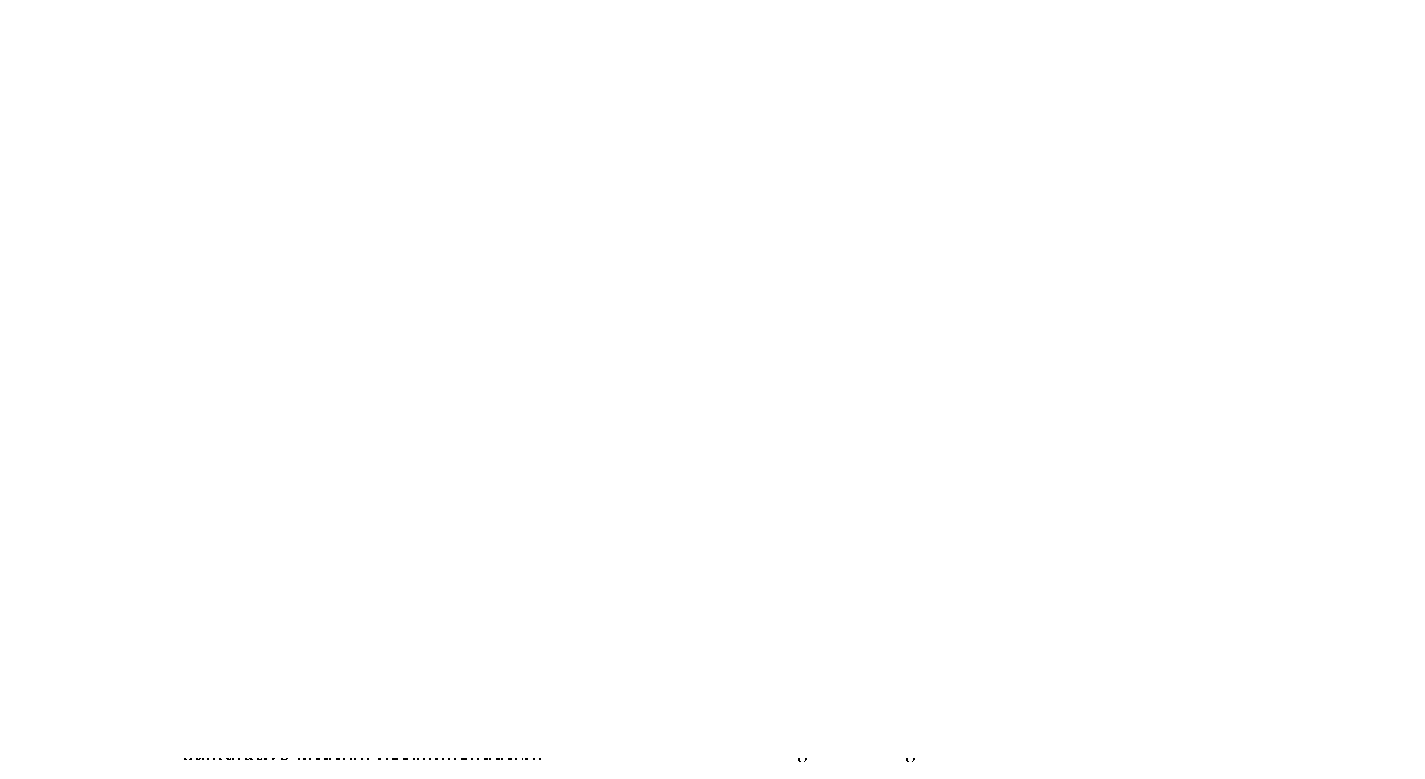
\includegraphics[width=4.5in]{./images/system.eps}
\vspace*{-.1in} \caption{Pipeline Design }\label{fig:system}
\vspace*{-.2in}
\end{figure}

\section{Pipeline}

\ceg{Discuss current system first. If you want to keep the decisions points
that led to the current architecture, make it a subsection.}
In this section we provide a high level description of the pipeline(system) 
design for big data analysis regarding TREC KBA the Stream Slot Filling (SSF) 
task. Our pipeline of processing the corpus consists of a two layer indexing 
system main section in our system regarding indexing the corpus, We started 
off by trying to use the off-the-shelf tools for this task. Mainly we started 
by using Scala/Spark\cite{ferc11} to benefit from the parallelization 
performance there.  Spark was not as efficient as expected and the overhead 
was much more than tolerable. We tried to use Scala parallelization itself to 
do the job, and unfortunately it did not satisfy our needs, there was 
excessive memory overhead on map reduce jobs. We migrated the core of the 
system to Java Parallelism APIs and that was not good enough either, we wanted 
better. So we built our own parallel system which in actual performance had 
the least of overhead, the least memory consumption and the most robust memory 
model which avoided unpredictable CPU stalls on garbage collections in 
processing the corpus. In what follows we will describe each step of this 
evolution in details. Figure~\ref{fig:system} shows a schematic view of the 
system. The platform that we run our pipeline over was a 32 core server having 
64GB of memory.




% Note: Describe the algorithms of each phase
% Talk in abstract terms not implementation.
% Use formal representations (Math, SQL etc)

\subsection{Cumulative Citation Recommendation}

\ceg{This section should be structured as follows:
1: Introduce CCR (Motivation, Expectations)
2: Our high level approach
3: Discussion of our design (Like already discussed)
}
Regarding Cumulative Citation Recommendation we perform exact string matching 
and treat all the documents that mention an entity equally likely to be citable.
For future iterations of the paper we have ideas on how to score documents 
based on their likelihood of citation worthiness but for this iterations we 
treat all mentioning documents equally likely. One of the reasons for this is 
that in former TREC KBA reports \cite{JFrank12} there were observations of how 
non-mentioning documents have highly low chance of being citable in Wikipedia.
So we take on that and ignore non-citing documents. Regarding mentioning but 
garbage, neutral or central documents we produce more slot values which can be 
later on filtered out in the high accuracy filter section.

\subsection{Streaming Slot Filling}
\ceg{See the previous note.}
Stream slot filling is done by pattern matching documents with manually 
produced patterns for slots of interest. The way we do this is by observing a 
sentence that has a mention of the entity or one of its coreferences. An 
anchor word in the sentence related to the slot name is located and we match 
either left or right of the anchor word for potential slot values. 

\subsection{Post Processing Algorithm}

The SSF output of many extractions is noisy. The data contains duplicates and 
incorrect extractions. We can define rules to sanitize the output only using 
the information present in the SSF file. The file is processed in time order, 
in a tuple-at-a-time fashion to minimize the impact on accuracy. We define 
two classes of rules deduplication rules and inference rules.
